\documentclass{article}

%\usepackage[utf8]{inputenc}		% LuaTex do not need this
%\usepackage[T1]{fontenc}			% LuaTex do not need this
\usepackage{fontspec}				% LuaTex need this
\usepackage{lmodern}
\usepackage{comment}
\usepackage[a4paper]{geometry}
\usepackage{graphicx}
	\graphicspath{ {Bilder/} }

%%%%%%%%%%%%%%%%%%%%%%%%%%%%%%%%%%%%%%%%%%%%%%%%%%%%%%%%%%%%%%%%%%%%%%%%%%%%%%%%
%
% https://tex.stackexchange.com/questions/82993/how-to-change-the-name-of-document-elements-like-figure-contents-bibliogr
% https://tex.stackexchange.com/questions/186946/changing-the-autoref-name-for-chapter
%
%\usepackage[ngerman]{babel}		% LuaTex do not need this
\usepackage{polyglossia}
	\setdefaultlanguage[spelling=new]{german}
	\addto\captionsgerman{
		\renewcommand{\figurename}{Abbildung}
		\renewcommand{\figureautorefname}{Abbildung}
		\renewcommand{\equationautorefname}{Gleichung}
	}


%%%%%%%%%%%%%%%%%%%%%%%%%%%%%%%%%%%%%%%%%%%%%%%%%%%%%%%%%%%%%%%%%%%%%%%%%%%%%%%%
%
% LATEX Mathematical Symbols
% https://reu.dimacs.rutgers.edu/Symbols.pdf
% https://en.wikibooks.org/wiki/LaTeX/Mathematics
%
\usepackage{amssymb}
\usepackage{amsthm}
\usepackage{amsmath}

%%%%%%%%%%%%%%%%%%%%%%%%%%%%%%%%%%%%%%%%%%%%%%%%%%%%%%%%%%%%%%%%%%%%%%%%%%%%%%%%
%
% algorithm2e.sty — package for algorithms
% http://ctan.mirrors.hoobly.com/macros/latex/contrib/algorithm2e/doc/algorithm2e.pdf
%
\usepackage[
	ngerman,
	linesnumbered,
	boxed,
%	algochapter,
%	rightnl,
%	figure,
]{algorithm2e}
	% Then you can adjust the spacing between the body of the algorithm and its
	% caption through the command \SetAlCapSkip.
	\SetAlCapSkip{1em}
	% Restyling the caption in an algorithm created with algorithm2e
	% https://tex.stackexchange.com/questions/112294/restyling-the-caption-in-an-algorithm-created-with-algorithm2e/112295
	\SetAlgoCaptionSeparator{:}
	\renewcommand\AlCapFnt{\normalfont}
	% Algorithm2e modify line numbers
	% https://tex.stackexchange.com/questions/100145/algorithm2e-modify-line-numbers
	\SetNlSty{textbf}{}{:}
	% Sets the value of the space between the line numbers and the text, by default 1em.
	\SetNlSkip{2em}
	%\SetAlgoRefName{QXY}

%%%%%%%%%%%%%%%%%%%%%%%%%%%%%%%%%%%%%%%%%%%%%%%%%%%%%%%%%%%%%%%%%%%%%%%%%%%%%%%%
%
% TikZ
%
\usepackage{tikz}
	\usetikzlibrary{arrows.meta,graphs,shapes}
\usepackage{tkz-berge}
\usepackage{tkz-graph}
\makeatletter
\pgfmathdeclarefunction{alpha}{1}{%
	\pgfmathint@{#1}%
	\edef\pgfmathresult{\pgffor@alpha{\pgfmathresult}}%
}
%%%%%%%%%%%%%%%%%%%%%%%%%%%%%%%%%%%%%%%%%%%%%%%%%%%%%%%%%%%%%%%%%%%%%%%%%%%%%%%%
%
% https://www.dante.de/events/Archiv/dante2012/Programm/Vortraege/vortrag-ferber.pdf
%
\usepackage[
	breaklinks,
	colorlinks,
	linkcolor=black,
	urlcolor=black,
	citecolor=black,
	pdfencoding=auto,
]{hyperref}
%%%%%%%%%%%%%%%%%%%%%%%%%%%%%%%%%%%%%%%%%%%%%%%%%%%%%%%%%%%%%%%%%%%%%%%%%%%%%%%%
%
%
%
\usepackage{verbatim}
\usepackage{float}
\usepackage{subcaption}
	\captionsetup{subrefformat=parens}
\usepackage{rail}

%
% Längenangabe für die Einrückung der ersten Zeile eines neuen Absatzes.	
% https://golatex.de/wiki/%5Cparindent
%
\setlength{\parindent}{0mm}


%%%%%%%%%%%%%%%%%%%%%%%%%%%%%%%%%%%%%%%%%%%%%%%%%%%%%%%%%%%%%%%%%%%%%%%%%%%%%%%%
%
%
%
\title{Technische Informatik\\ Lösungen zu der Übung 5}

\author{
	Albert Kasdorf\and
	Georg Braun
}
\date{22.05.2018}



%%%%%%%%%%%%%%%%%%%%%%%%%%%%%%%%%%%%%%%%%%%%%%%%%%%%%%%%%%%%%%%%%%%%%%%%%%%%%%%%
%
%
%
\begin{document}

\maketitle

\section*{Aufgabe 39 (CFGs)}
Betrachten Sie die CFG GSE in \autoref{fig:compilerbau_abbildung_11_18} und das Wort

\begin{equation*}
	\text{w = IDENT "=" NUMBER "*" IDENT "*" NUMBER ";".}
\end{equation*}

\begin{figure}[h]
	\centering
	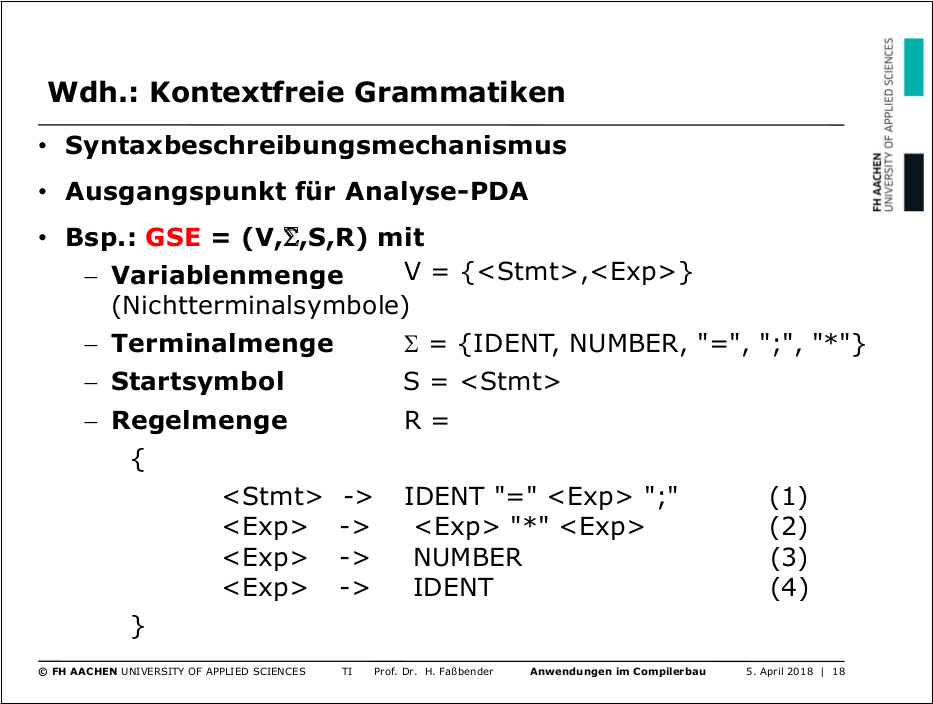
\includegraphics[width=0.75\linewidth]{Compilerbau_Abbildung_11_18}
	\caption{Wdh.: Kontextfreie Grammatiken}
	\label{fig:compilerbau_abbildung_11_18}
\end{figure}

a) Geben Sie ein Syntaxdiagramm an, das die durch GSE erzeugte Sprache beschreibt.

\begin{rail}
	statement : 'IDENT' '=' exp ';'
\end{rail}

\begin{rail}
	exp : exp '*' exp | 'NUMBER' | 'IDENT'
\end{rail}


b) Geben Sie eine Linksableitung von w an.


c) Geben Sie eine Rechtsableitung von w an.


\section*{Aufgabe 40 (Mehrdeutige CFGs)}
Geben Sie eine CFG und ein Wort w an, so dass es für das Wort w zwei verschiedene Linksableitungen zu w gibt und beweisen Sie Ihre Aussage durch Angabe der beiden Linksableitungen zu w.

Zeichnen Sie zu jeder Linksableitung den zugehörigen Syntaxbaum.


\section*{Aufgabe 41 (CNF)}

Geben Sie eine Typ 2-Grammatik an, die die folgende Sprache erzeugt und transformieren Sie
diese in CNF:

\begin{equation*}
	\left\{a^n b^n c^m \mid n, m \geq 1\right\}.
\end{equation*}


\section*{Aufgabe 42 (Top-Down-Analyserechnung)}

a) Geben Sie eine CFG an, die die Menge der nichtleeren Palindrome (Wort gleich dem gespiegelten Wort) über dem Alphabet $\Sigma = \left\{a, b, c\right\}$ erzeugt. Bsp.: $w=abccba$ ist in der zu erzeugenden Menge.

b) Geben Sie eine Top-Down Analyserechnung des Top-Down Analyseautomaten zur CFG aus Teil a) für das Wort $w=abccba$ an, die erfolgreich ist.

c) Geben Sie eine Top-Down Analyserechnung des Top-Down Analyseautomaten zur CFG aus Teil a) für das Wort $w=abccba$ an, die erfolglos abbricht.


\section*{Aufgabe 43 (Durchschnitt Typ 2-Sprachen)}

Beweisen oder widerlegen Sie, dass der Schnitt von L 1 und L 2 aus Aufgabe 37 und Aufgabe 38 Typ 2 ist.


Was bedeutet das für die Abschlusseigenschaften der Typ 2-Sprachen?


\section*{Aufgabe 44 (Typ 1-Sprache)}

Zeigen Sie, dass die Sprache $L = \left\{a^m b^m c^m \mid m \geq 1\right\}$ vom Typ 1 ist.


\end{document}